\documentclass[PREyA.tex]{subfiles}

\usepackage{tikz}
\usetikzlibrary{automata,positioning}
\providecommand{\abs}[1]{\left\lvert#1\right\rvert}
\begin{document}

\chapter{Cadenas de Markov en tiempo continuo}
\section{Introducción}
\begin{defi}
Se dice que una cadena en tiempo continuo es de Markov si verifica la propiedad de Markov, es decir, si $\forall n \geq 2$ $\forall 0\leq t_1 < \dotsc < t_n$ y $\forall i_1,\dotsc,i_n\in S$ se verifica
$$
P[X_{t_n} = i_n \mid X_{t_1}=i_1,\dotsc,X_{t_{n-1}}=i_{n-1}] = P[X_{t_n} = i_n \mid X_{t_{n-1}} = i_{n-1}]
$$
\end{defi}
\begin{defi}
A los valores $i_1,\dotsc,i_{n-1}$ se les denomina \textbf{historia} y, en particular, $i_{n-1}$ es el \textbf{pasado inmediato}.
\end{defi}
\begin{example}
El proceso de Poisson verifica la propiedad markoviana. Se deduce trivialmente a partir de incrementos independientes.
\end{example}
\begin{defi}
Podemos considerar $p_{ij}^{(s,t)}$ a la probabilidad de que el proceso en el instante $t$ esté en $j$ condicionado a que en el instante $s$ estaba en $i$, es decir,
$$
p_{ij}^{(s,t)} = P[X_t =j \mid X_s = i]
$$
Luego podemos considerar $P_{st} = (p_{ij}^{(s,t)})$ con $i,j \in S$ y para $0\leq s \leq t$.
\end{defi}
\begin{nota}
Supondremos en adelante que se verifica la propiedad de homogeneidad en el tiempo, es decir, que las $p_{ij}^{(s,t)}$ son funciones de la diferencia en el tiempo $t-s$. 
\end{nota}
\begin{nota}
Bajo la asunción anterior podemos escribir simplemente $P_t = (p_{ij}^{(0,t)})$, pues
$$
P[X(t+s)=j \mid X(s)=i] = P[X(t)=j\mid X(0)=i]
$$
\end{nota}
\newpage
\begin{prop}
Se verifican las siguientes propiedades
\begin{itemize}
\item $P_0 = I_{|S|\times |S|}$.
\item $P_t$ es una matriz estocástica.
\item Verifica las ecuaciones de Chapman Kolmogorov, es decir
$$
P_{t+s}=P_tP_s \quad \forall s,t\geq 0
$$
\end{itemize}
\end{prop}
\begin{dem} Tenemos
\begin{itemize}
\item $p_{ij}(0) = P[X(0)=j\mid X(0)=i]$.
\item Sumamos directamente
\begin{align*}
1 &= P[X(t)\in S \mid X(0)=i] \\
&= \sum_{j \in S} P[X(t)=j \mid X(0)=i]\\
&=\sum_{j\in S} p_{ij}(t)
\end{align*}
\item 
\begin{align*}
p_{ij}(t+s) &= P[X(t+s) =j \mid X(0)=i]\\
& = P[X(t+s)=j, X(t)\in S \mid X(0)=i]\\
&=\sum_{k \in S} P[X(t+s)=j, X(t)=k \mid X(0)=i]\\
&=\sum_{k\in S} P[X(t) = k  \mid X(0)=i] P[X(t+s) = j \mid X(0)=i, X(t)=k]\\
&=\sum_{k\in S} P[X(t) = k  \mid X(0)=i] P[X(t+s) = j \mid  X(t)=k]\\
&=\sum_{k\in S} p_{ik}(t) P[X(s) = i \mid  X(0)=k]\\
&=\sum_{k\in S} p_{ik}(t) p_{kj}(s) 
\end{align*}
Por tanto, $P_{t+s} = P_t P_s$.
\end{itemize}

\end{dem}
\begin{prop}
El conjunto $\{P_t\}_{t\geq 0}$ tiene estructura de semigrupo con la operación producto.
\end{prop}
\begin{nota}
Vamos a suponer por simplicidad que todos los semigrupos son standar, es decir, 
$$
\lim_{t\to0} P_t = I
$$
\end{nota}

\begin{nota}
Describir una cadena de Markov a partir de sus matrices de probabilidad y el estado inicial puede ser costoso en la práctica.
\end{nota}
\begin{defi}
Definimos la matriz de generadores siempre que tenga sentido
$$
G:= \lim_{h\to 0^+} \frac{P_h -I }{h} 
$$
\end{defi}
\begin{prop}
Bajo la hipótesis de que los semigrupos son standar, se tiene que
$$
G= (p_{ij}'(0))
$$
\end{prop}

\begin{prop}[Interpretación de $G$] 
\begin{itemize}
\item[]
\item Elementos diagonales $g_{ii}$. Sea $T_i$ el tiempo de permanencia en un estado $i$. Entonces $T_i \sim Exp(-g_ii)$
\item Elementos extradiagonales $g_{ij}$ $i\neq j$. 
\end{itemize}
\end{prop}
\begin{dem}
Por la homogeneidad en el tiempo podemos suponer que estamos en el instante $t=0$. Para la primera part vamos a calcular el complementario la función de distribución
\begin{align*}
P[T_i > t] &\approx P[X_{i/N} =i \colon \forall i = 1,\dotsc tN, \forall N \mid X_0 = i]\\
&= \prod_{i=1}^{Nt} P[X_{i/N}=i\mid X_{(i-1)/N}=i]\\
&= p_{ii}\left(\frac{1}{N}\right)^{tN} \\
&= \left(1+\frac{g_{ii}}{N}+o(1/N)\right)^{tN} \longrightarrow e^{-g_{ii} t}
\end{align*}
Para la segunda parte consideramos
\begin{align*}
P[N(t+h) = j \mid N(t)=i \text{ y hay salto}] &= \frac{P[N(t+h) = j, N(t)=i \text{ y hay salto}]}{P[N(t)=i \text{ y hay salto}]}\\
&=\frac{P[N(t)=i]P[N(t+h)=j\mid N(t)=i,\;i\neq j}{P[N(t)=i]P[\text{Hay salto}\mid N(t)=i]}\\
&=\frac{P[N(t)=i]p_{ij}(h)}{P[N(t)=i]\sum_{k\neq i} P[N(t+h)=k\mid N(t)=i]}\\
&=\frac{p_{ij}(h)}{\sum_{k\neq i} p_{ik}(h)}\\
&= \frac{g_{ij}h+o(h)}{\sum_{k\neq i} g_{ik}h+o(h)}\\
&\overset{h\to 0}{\approx} -\frac{g_{ij}}{g_{ii}}
\end{align*}
Hemos calculado la probabilidad de saltar al estado $j$ suponiendo que estamos en $i$.
\end{dem} 
\begin{nota}
La representación de una cadena de Markov en tiempo continuo a través de un grafo se realiza escribiendo sobre las flechas los elementos de $G$, salvo los loops que no se escriben. 

Por ejemplo, sea una cadena de Markov dada por la matriz
$$
G= 
\begin{pmatrix}
-a & a\\
b & -b
\end{pmatrix}
$$
Entonces el grafo asociado es
\begin{center}
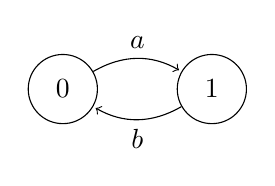
\begin{tikzpicture}
	% Draw the states
	\node[state]             (1) {$0$};
	\node[state, right=of 1] (2) {$1$};
    % Connect the states with arrows
	\draw[every loop]
		(1) edge[bend left, auto=left] node {$a$} (2)
		(2) edge[bend left, auto=left] 	   node {$b$} (1);
\end{tikzpicture}
\end{center}
\end{nota}
\end{document}
